\documentclass[nojss]{jss}\usepackage[]{graphicx}\usepackage[]{color}
%% maxwidth is the original width if it is less than linewidth
%% otherwise use linewidth (to make sure the graphics do not exceed the margin)
\makeatletter
\def\maxwidth{ %
  \ifdim\Gin@nat@width>\linewidth
    \linewidth
  \else
    \Gin@nat@width
  \fi
}
\makeatother

\definecolor{fgcolor}{rgb}{0.345, 0.345, 0.345}
\newcommand{\hlnum}[1]{\textcolor[rgb]{0.686,0.059,0.569}{#1}}%
\newcommand{\hlstr}[1]{\textcolor[rgb]{0.192,0.494,0.8}{#1}}%
\newcommand{\hlcom}[1]{\textcolor[rgb]{0.678,0.584,0.686}{\textit{#1}}}%
\newcommand{\hlopt}[1]{\textcolor[rgb]{0,0,0}{#1}}%
\newcommand{\hlstd}[1]{\textcolor[rgb]{0.345,0.345,0.345}{#1}}%
\newcommand{\hlkwa}[1]{\textcolor[rgb]{0.161,0.373,0.58}{\textbf{#1}}}%
\newcommand{\hlkwb}[1]{\textcolor[rgb]{0.69,0.353,0.396}{#1}}%
\newcommand{\hlkwc}[1]{\textcolor[rgb]{0.333,0.667,0.333}{#1}}%
\newcommand{\hlkwd}[1]{\textcolor[rgb]{0.737,0.353,0.396}{\textbf{#1}}}%
\let\hlipl\hlkwb

\usepackage{framed}
\makeatletter
\newenvironment{kframe}{%
 \def\at@end@of@kframe{}%
 \ifinner\ifhmode%
  \def\at@end@of@kframe{\end{minipage}}%
  \begin{minipage}{\columnwidth}%
 \fi\fi%
 \def\FrameCommand##1{\hskip\@totalleftmargin \hskip-\fboxsep
 \colorbox{shadecolor}{##1}\hskip-\fboxsep
     % There is no \\@totalrightmargin, so:
     \hskip-\linewidth \hskip-\@totalleftmargin \hskip\columnwidth}%
 \MakeFramed {\advance\hsize-\width
   \@totalleftmargin\z@ \linewidth\hsize
   \@setminipage}}%
 {\par\unskip\endMakeFramed%
 \at@end@of@kframe}
\makeatother

\definecolor{shadecolor}{rgb}{.97, .97, .97}
\definecolor{messagecolor}{rgb}{0, 0, 0}
\definecolor{warningcolor}{rgb}{1, 0, 1}
\definecolor{errorcolor}{rgb}{1, 0, 0}
\newenvironment{knitrout}{}{} % an empty environment to be redefined in TeX

\usepackage{alltt}
\usepackage[sc]{mathpazo}
\usepackage{geometry}
\geometry{verbose,tmargin=2.5cm,bmargin=2.5cm,lmargin=2.5cm,rmargin=2.5cm}
\setcounter{secnumdepth}{2}
\setcounter{tocdepth}{2}
\usepackage{breakurl}
\usepackage{hyperref}
\usepackage[ruled, vlined]{algorithm2e}
\usepackage{mathtools}
\usepackage{hyperref}
\usepackage{color}
\usepackage{float}
\usepackage{placeins}
\usepackage{mathrsfs}
\usepackage[toc,page]{appendix}
\usepackage{multirow}
\usepackage{amsmath}
\usepackage{breqn}
\usepackage[demo]{graphicx}% "demo" to make example compilable without .png-file
\usepackage[font=small,labelfont=bf]{caption}
\usepackage{lipsum}

\usepackage{booktabs}
\newcommand{\head}[1]{\textnormal{\textbf{#1}}}
%% \usepackage{mathbbm}
\DeclareMathOperator{\sgn}{sgn}
\DeclareMathOperator*{\argmax}{\arg\!\max}

\title{\bf{SWS Population Domain} }

\author{Francesca Rosa\\ Food and Agriculture
    Organization \\ of the United Nations\\}

\Plainauthor{Francesca Rosa}

\Plaintitle{faoswsImputation: A sub-module for the imputation of missing time
series data in the Statistical Working System - Processed items}

\Shorttitle{Derived item production}

\Abstract{

   Population: this document contains information on the overall workflow to populate the new population datasets stored in the \code{SWS}. It replies to many questions as for example: why have these datasets been created? How can these datasets be updated when a new realise from the data-source is available?  \\

}

\Keywords{Population, World Population Prospects, World Urbanization Prospect}
\Plainkeywords{Population, World Population Prospects, World Urbanization Prospect}

\Address{
  Francesca Rosa\\
  Economics and Social Statistics Division (ESS)\\
  Economic and Social Development Department (ES)\\
  Food and Agriculture Organization of the United Nations (FAO)\\
  Viale delle Terme di Caracalla 00153 Rome, Italy\\
  E-mail: \email{Francesca.Rosa@fao.org}\\
  URL: \url{https://svn.fao.org/projects/SWS/RModules/faoswsProduction/}
}
\IfFileExists{upquote.sty}{\usepackage{upquote}}{}
\begin{document}

\section{Purpose}
Several statistical processes already embedded in the \code{SWS} depend on the Population. For example, the per capita Dietary Energy Supply, by definition, can be computed as long as we dispose of reliable population data.

In addition, since many Statistical processes depend on the Population, it is extremely important to ensure that all those processes point to the same Population variables in order to ensure the compliance and the comparability between different environments in the \code{SWS}.


The purpose of the recent review of the Population domain is to identify a unique source for Population data.

This paragraph contains information about the Population data already stored in the \code{SWS} in the dataset \textit{Population}.

In particular, the dataset \code{Population} contains three elements:

\begin{itemize}
\item{\textit{Total Population} [\code{element-code 11}]}
\item{\textit{Food balance sheets population},  [\code{element-code 21]}
\item{\textit{Weighted Total Population},  [\code{element-code 511]}
\end{itemize}

Apparently, these variables have not been updated anymore, and we do not dispose of sufficient metadata to rebuild the statistical processes performed to compute this figures.


\section{The new UNPD dataset}

It has been agreed that the only source for Population data is the \textbf{United Nations Population Departement} (UNPD) who disseminates the \textit{World Population Prospects} (WPP) and the \textit{World Urbanization Prospect} (WUP).
The UNPD database can be directly accessed from the \href{http://www.un.org/en/development/desa/population/publications/database/index.shtml}{UNDP URL}.


The elements we inherit from the UNPD data-source are:

\begin{itemize}
\item{Total population  (WPP), [\code{element-code: 511]}
\item{Female population (WPP), [\code{element-code: 513]}
\item{Male population (WPP), [\code{element-code: 512]}
\item{Urban population (WUP), [\code{element-code: 561]}
\item{Rural population (WUP), [\code{element-code: 551]}
\end{itemize}

These variables are already published on FAOSTAT. In order to ensure the complince in terms of classifications (berween FAOSTAT and the \code{SWS}) the same element-codes have been used to stored these elements in the \code{SWS}.

\textcolor{red}{\textbf{IMPORTANT NOTE: }} please note that the \textbf{new release of the World Population Prospects and the World Urbanization Prospects may not occur at the same time}. The implication of this misalignment in the release of the WPP and the WUP is, mainly, the possible misalignment of the Regions that might have been designed in different moments. For this reason, we suggest to look separately at the following documents:

\begin{itemize}
\item{\href{https://esa.un.org/unpd/wpp/General/Files/Definition_of_Regions.pdf}{World Population Prospects: The 2017 Revision - CLASSIFICATION OF COUNTRIES BY REGION, INCOME GROUP
AND SUBREGION OF THE WORLD }}
\item{\href{https://esa.un.org/unpd/wup/CD-ROM/WUP2014_DOCUMENTATION/WUP2014_DEFINITION_OF_MAJOR_AREAS_AND_REGIONS.pdf}{World Urbanization Prospects: The 2014 Revision - CLASSIFICATION OF COUNTRIES BY MAJOR AREA
AND REGION OF THE WORLD AND INCOME GROUP}}
\end{itemize}



The World Population Prospects also contains long terms projection of the Total, Female and Male Population. The projections we have included in the \code{SWS} are under the assumptions of "Medium variant fertility" \footnote{Additional information is available in the UNPD document: \href{https://esa.un.org/unpd/wpp/Publications/Files/WPP2017_Methodology.pdf}{Methodology of the United Nations Population Estimates and Projections, 2017 Revision}}.

All this information is stored in the metadata in order to support the users to properly interpret data.
In particular, the metadata associated to every single figure contains information on:

\begin{itemize}
\item{the data source which can be either the \textit{World Population Prospect} (WPP) or the \textit{World Urbanization Prospect} (WUP); }
\item{the year of the last realise;}
\item{if the figure is an estimation or a projection and, in this latter case, the method used to compute the projection, so far \textit{Medium Variant}}
\end{itemize}



\begin{center}
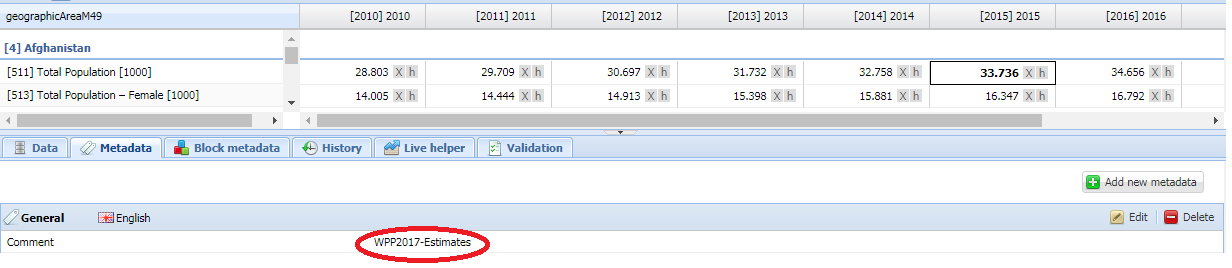
\includegraphics{metadata.PNG}
\captionof{figure}{Metadata example}
\end{center}


Two dataset has been created to host the UNPD population data:
\begin{itemize}
\item{\textbf{Source Population UNPD}, this dataset represents a clone of the data disseminated by UNPD. It basically contains all the UNPD data. The reason why we decided to create this dataset is that despite both UNPD and FAO support the same international classification for the geographic area, the perfect compliancy is ensured only at country level. We verify that there is no match in terms of M49 codes for Regions or Country Groups. We decided to host in any case all the data about Regions and Aggregates since \textit{countries or areas listed individually are only those with 90,000 inhabitants or more in 2017; the rest are included in the aggregates but are not listed separately.}\footnote{UNPD}}
\item{\textbf{Population UNPD}, this detasets is the \textit{operational} one. It contains only the M49 codes supported by the FAO. This means that all the other statistical processes embedded in the \code{SWS} should point to this dataset.}
\end{itemize}


\section{How to update new UNPD datasets}

UNPD Data must be manually downloaded from the \href{http://www.un.org/en/development/desa/population/publications/database/index.shtml}{UNPD download page}. A routine has been created to structure the data in order to be hosted by the \code{SWS}. This routine depends on the structure of the files downloaded and can be re-used as long as the UNPD files have the same template.

Some additional operations have to be performed in order to locally store the data in a way that is suitable to be imported in the \code{SWS}.
\begin{enumerate}
\item{The first step is to create, within the R work directory, the folder structure to host the UNPD data. The R routine contains the path to access to each file so it is important to reproduce exactly the same folder and sub-folder structure unless the path is properly changed.





\begin{center}
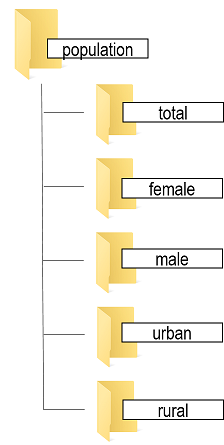
\includegraphics[width=6cm, height=11cm]{folderStructure}
\captionof{figure}{Folder structure}
\end{center}
}
\item{As already mentioned, UNPD data may come from the \textit{World Population Prospects} (Total population, Female and Male population) and from the \textit{World Urbanization Prospect} (Rural and Urban population). Data coming from the  \textit{World Population Prospects} contains long terms projections which are usually stored in a separated excel sheet. The second step is to extract from the downloaded excel files the proper csv files that can be imported into R to be reshaped and saved in the \code{SWS}



\begin{center}
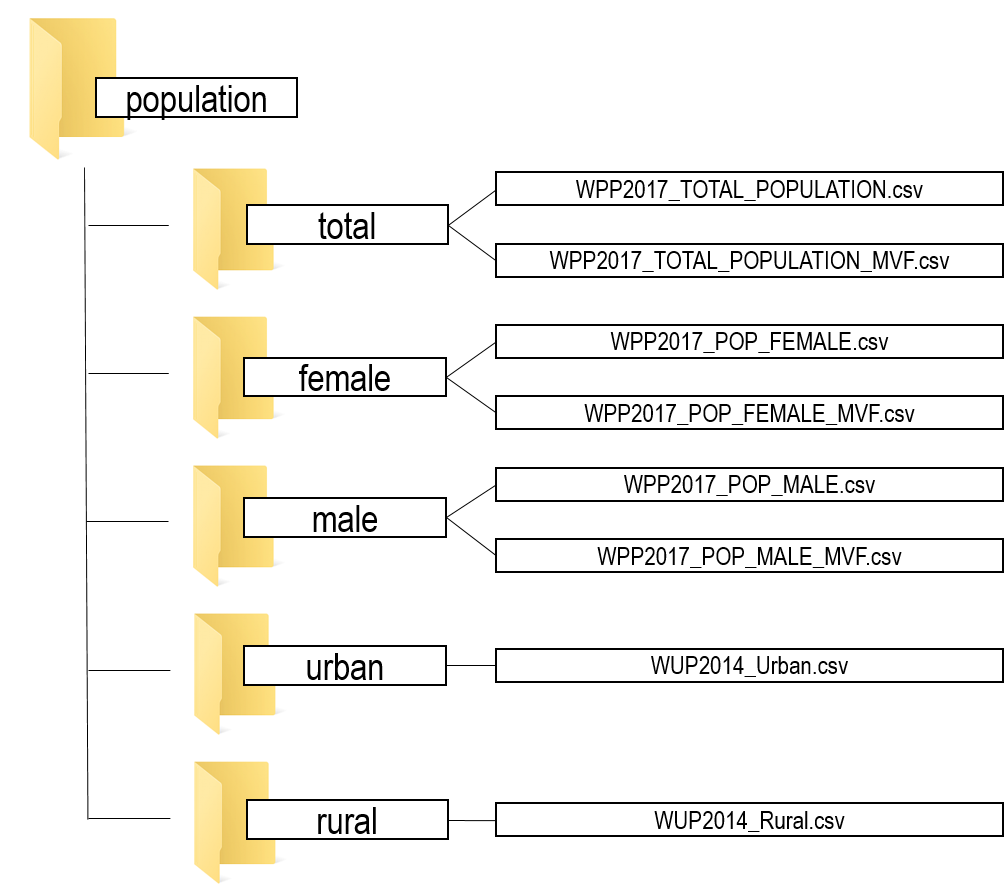
\includegraphics[width=13cm, height=11cm]{structureFiles}
\captionof{figure}{The files WPP2017_TOTAL_POPULATION_MVF.csv, PP2017_TOTAL_FEMALE_MVF.csv, PP2017_TOTAL_MALE_MVF.csv contains the Medium Fertility Variant projections.}
\end{center}





}
\item{Clean the csv files: delete the initial colums, rename the \textit{Area} column as reported in the following picture.

\begin{center}
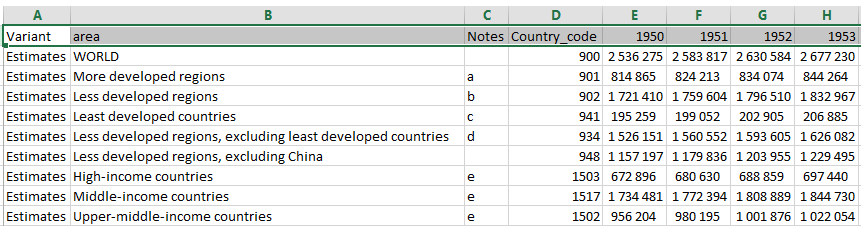
\includegraphics{CSV.PNG}
\captionof{figure}{CSV structure example}
\end{center}
}

\item{Open a new session on the \code{SWS} on the dataset \textit{Source UNPD population}. Create a new token using the only available plugin labelled \textbf{Population Token}. The token is obtained clicking on the \textit{"New debug session"}.

\begin{center}
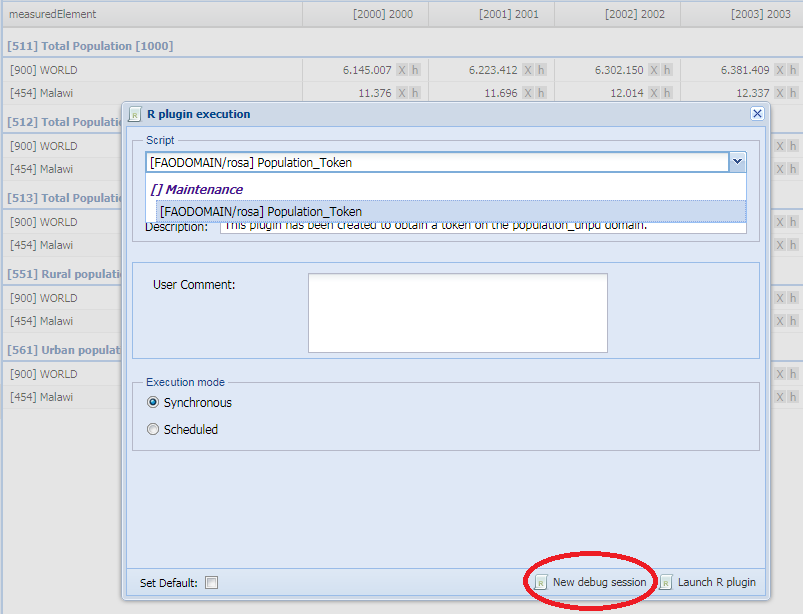
\includegraphics{SourceToken.PNG}
\captionof{figure}{Create a Token from the dataset, Source UNPD population}
\end{center}
}

\item{Use the token to perform the sub-routine stored in the Rstudio \textit{Population project}: \textbf{convertUNPDdata.R}.

This routine:
\begin{itemize}
\item{assign the \code{SWS} elements to the different UNPD variables;}
\item{assign \code{SWS} flags;}
\item{build the \code{SWS} metadata file. Please specify in the routine the version of both the WPP and WUP (line 1-2), For example at the moment we have \textit{"WPP2017"} and \textit{"WUP2014"};}
\item{populate the Source UNPD population dataset with the new figures.}
\end{itemize}

}

\end{enumerate}




Once the Source UNPD Population dataset has been populated, it is possible to open a new session directly in the \code{SWS} on the \textbf{UNPD population} dataset and run the \textbf{UNPD synchronization plugin} that populates the \textit{operational dataset} with only the M49 compliant geographic codes.



\end{document}
